\documentclass[reprint,amsmath,amssymb,aps,prl,floatfix,onecolumn]{revtex4-2}
\usepackage[brazilian]{babel}
\usepackage[T1]{fontenc}
\usepackage{graphicx}% Include figure files
\usepackage{dcolumn}% Align table columns on decimal point
\usepackage{bm}% bold math
\usepackage{multirow}
\usepackage{subfigure}
\usepackage{color}
\usepackage[normalem]{ulem}
\usepackage{float}
\usepackage{cprotect}
\usepackage{colortbl}

\begin{document}
\begin{titlepage}					% Inicia capa
	
	% Comando para régua horizontal estilosa:
	\newcommand{\sectionline}{%
		\nointerlineskip \vspace{\baselineskip}%
		\hspace{\fill}\rule{1\linewidth}{0.8pt}\hspace{\fill}%
		\par\nointerlineskip \vspace{\baselineskip}
	}
	
	\begin{center}
		
		% Parte de cima da página:
		
\includegraphics[scale=0.4]{LogoITA.jpg}
		
		{\large
			\textsc{Instituto Tecnol\'ogico de Aeron\'autica}\\
			\textsc{Divis\~ao de Ci\^encias Fundamentais}\\
			\textsc{Departamento de F\'isica}\\
		}
		
		\vspace*{\fill}			% Centraliza texto verticalmente na pagina

		

		\sectionline
		
		% Título
		\textsc{\LARGE \bfseries E03 -- Filtros RC Passa-Alta e Passa-Baixa}\\

		\sectionline

		\begin{flushleft}
			\emph{\textbf{Autores:}} Gael Vinícius Maia Sampaio, Jônatas Augusto de Paula, José Guilherme Correia de Menezes, Paulo Otávio Portela Santana, Pedro Diogo Leal Arteiro  \\
			\emph{\textbf{Grupo/turma:}} Grupo 5/Turma 2
		\end{flushleft}


		\vspace*{\fill}

		% Titulo
		\textsc{\Large Relatório de FIS-46 -- Laboratório de Física} \\

			\textsc{Prof. Argemiro Soares da Silva Sobrinho}
		
		\vfill
		
		% Parte de baixo da página
		{\large \today}				
		
	\end{center}
	
\end{titlepage}

\newpage

\title{Filtros RC Passa-Alta e Passa-Baixa}

\author{Gael Vinícius Maia Sampaio}
\affiliation{Instituto Tecnológico de Aeronáutica, S\~{a}o José dos Campos, Brasil}
\author{Jônatas Augusto de Paula}
\affiliation{Instituto Tecnológico de Aeronáutica, S\~{a}o José dos Campos, Brasil}
\author{José Guilherme Correia de Menezes}
\affiliation{Instituto Tecnológico de Aeronáutica, S\~{a}o José dos Campos, Brasil}
\author{Paulo Otávio Portela Santana}
\affiliation{Instituto Tecnológico de Aeronáutica, S\~{a}o José dos Campos, Brasil}
\author{Pedro Diogo Leal Arteiro}
\affiliation{Instituto Tecnológico de Aeronáutica, S\~{a}o José dos Campos, Brasil}

\date{\today}

\begin{abstract}
Este trabalho determina experimentalmente as curvas de resposta em frequência (ganho e fase) de dois filtros RC de primeira ordem, passa-altas (saída sobre o resistor) e passa-baixas (saída sobre o capacitor), montados com $R=1{,}5\,\text{k}\Omega$ e $C=0{,}1\,\mu\text{F}$ nominais, para 16 frequências entre $10\,\text{Hz}$ e $40\,\text{kHz}$, usando um osciloscópio digital de duplo canal com medida automática de tensão pico a pico e defasagem. As curvas medidas de ganho e fase acompanham de perto o modelo de impedância complexa em toda a faixa estudada, com resíduos de ganho tipicamente abaixo de $1\%$ e resíduos de fase abaixo de $1^\circ$ na maior parte dos pontos. A frequência de corte determinada experimentalmente por interpolação do cruzamento em $-3\,\text{dB}$ foi de $1081\,\text{Hz}$ (passa-altas) e $1085\,\text{Hz}$ (passa-baixas), em excelente acordo com o valor teórico $f_c=1061\pm119\,\text{Hz}$. Duas limitações de coleta de dados são discutidas abertamente: dois pontos do filtro passa-altas ($800$ e $1300\,\text{Hz}$) tiveram apenas o ganho medido, sem captura da defasagem, e o ponto de $10\,\text{Hz}$ do mesmo filtro apresentou um valor de fase com sinal invertido em relação à tendência dos demais pontos, atribuído a uma provável ambiguidade do algoritmo de medida automática do osciloscópio sob sinal fortemente atenuado e ruidoso.
\end{abstract}

\maketitle

\section{Resultados e discussão}

Os dois circuitos estudados são filtros RC de primeira ordem montados sobre um quadro de conexões com resistor de filme $R=1{,}5\,\text{k}\Omega$ (tolerância de fabricação adotada de $\pm5\%$, valor nominal não conferido com multímetro nesta prática) e capacitor cerâmico $C=0{,}1\,\mu\text{F}$ (tolerância adotada de $\pm10\%$), excitados por um gerador de funções em onda senoidal com acoplamento CA no osciloscópio digital Tektronix TBS 1052B-EDU. No filtro passa-altas, o canal 1 (CH1) foi conectado à saída do gerador (tensão de entrada $V_e$) e o canal 2 (CH2), ao resistor $R$ (tensão de saída $V_s$); no filtro passa-baixas, trocou-se a posição de $R$ e $C$ no circuito, de modo que $V_s$ passa a ser medida sobre o capacitor. Para tensões harmônicas, a Lei de Ohm generalizada fornece o ganho complexo $V_s/V_e$; para o passa-altas,
\begin{equation}
	\label{eq:ganho_pa}
	G_{PA}=\frac{\omega RC}{\sqrt{1+(\omega RC)^2}}, \qquad \Phi_{PA}=\arctan\!\left(\frac{1}{\omega RC}\right),
\end{equation}
e para o passa-baixas,
\begin{equation}
	\label{eq:ganho_pb}
	G_{PB}=\frac{1}{\sqrt{1+(\omega RC)^2}}, \qquad \Phi_{PB}=-\arctan(\omega RC),
\end{equation}
com $\omega=2\pi f$ \cite{Nussenzveig1997,Malvino2008}. Em ambos os casos, a frequência de corte $f_c$, definida pelo ponto em que o ganho cai a $1/\sqrt{2}$ ($-3\,\text{dB}$), é dada por $f_c=1/(2\pi RC)$, com incerteza propagada das tolerâncias de $R$ e $C$ pela regra usual de propagação de erros \cite{Vuolo1996}; para os componentes nominais acima, $f_c=1061\pm119\,\text{Hz}$.

Para cada frequência, $V_e$ e $V_s$ (tensão pico a pico) e a defasagem $\Phi=\text{Fase:Ch1-Ch2}$ foram lidos diretamente do quadro de medidas automáticas sobreposto à tela do osciloscópio, com incerteza de leitura adotada como $\pm1$ no último algarismo exibido pelo instrumento (por exemplo, $4{,}99\pm0{,}01\,\text{V}$ ou $60{,}9\pm0{,}1^\circ$), na ausência de uma especificação de acurácia do fabricante disponível para esta prática. O ganho $G=V_s/V_e$ e sua versão em decibéis, $G_{dB}=20\log_{10}G$, foram calculados com incerteza propagada da mesma forma \cite{Vuolo1996}. As Tabelas~\ref{tab:pa} e \ref{tab:pb} apresentam os dados brutos e as grandezas calculadas para os filtros passa-altas e passa-baixas, respectivamente, nas 16 frequências do roteiro.

\begin{table}[htb]
	\caption{\label{tab:pa} Dados brutos e grandezas calculadas do filtro passa-altas: tensão de entrada $V_e$ e de saída $V_s$ (pico a pico), defasagem $\Phi=$Fase:Ch1$-$Ch2, ganho $G=V_s/V_e$ e ganho em dB. $^\dagger$Defasagem não capturada nessa frequência (quadro de fase indisponível na tela salva, sem imagem alternativa); valor mostrado é a estimativa teórica da Eq.~\eqref{eq:ganho_pa}, não uma medida.}
	\begin{tabular}{cccccc}
		\hline\hline
		$f$ (Hz) & $V_e$ (V) & $V_s$ (V) & $\Phi$ (\textdegree) & $G$ & $G_{dB}$ (dB) \\ \hline
		10 & $4{,}11\pm0{,}01$ & $0{,}052\pm0{,}000$ & $-86{,}8\pm0{,}1$ & $0{,}013\pm0{,}000$ & $-37{,}94\pm0{,}03$ \\
		30 & $4{,}91\pm0{,}01$ & $0{,}150\pm0{,}001$ & $93{,}0\pm0{,}1$ & $0{,}031\pm0{,}000$ & $-30{,}30\pm0{,}06$ \\
		60 & $4{,}99\pm0{,}01$ & $0{,}290\pm0{,}001$ & $86{,}8\pm0{,}1$ & $0{,}058\pm0{,}000$ & $-24{,}71\pm0{,}03$ \\
		100 & $5{,}02\pm0{,}01$ & $0{,}471\pm0{,}001$ & $85{,}2\pm0{,}1$ & $0{,}094\pm0{,}000$ & $-20{,}55\pm0{,}03$ \\
		300 & $5{,}06\pm0{,}01$ & $1{,}370\pm0{,}010$ & $74{,}7\pm0{,}1$ & $0{,}271\pm0{,}002$ & $-11{,}35\pm0{,}07$ \\
		600 & $4{,}99\pm0{,}01$ & $2{,}430\pm0{,}010$ & $60{,}9\pm0{,}1$ & $0{,}487\pm0{,}002$ & $-6{,}25\pm0{,}04$ \\
		800 & $19{,}20\pm0{,}10$ & $11{,}600\pm0{,}100$ & $53{,}0^\dagger$ & $0{,}604\pm0{,}006$ & $-4{,}38\pm0{,}09$ \\
		1000 & $4{,}95\pm0{,}01$ & $3{,}400\pm0{,}010$ & $46{,}6\pm0{,}1$ & $0{,}687\pm0{,}002$ & $-3{,}26\pm0{,}03$ \\
		1300 & $19{,}20\pm0{,}10$ & $14{,}600\pm0{,}100$ & $39{,}2^\dagger$ & $0{,}760\pm0{,}007$ & $-2{,}38\pm0{,}07$ \\
		2000 & $5{,}02\pm0{,}01$ & $4{,}380\pm0{,}010$ & $27{,}4\pm0{,}1$ & $0{,}873\pm0{,}003$ & $-1{,}18\pm0{,}03$ \\
		3000 & $4{,}99\pm0{,}01$ & $4{,}690\pm0{,}010$ & $20{,}3\pm0{,}1$ & $0{,}940\pm0{,}003$ & $-0{,}54\pm0{,}03$ \\
		6000 & $4{,}99\pm0{,}01$ & $4{,}900\pm0{,}010$ & $10{,}3\pm0{,}1$ & $0{,}982\pm0{,}003$ & $-0{,}16\pm0{,}02$ \\
		10000 & $19{,}80\pm0{,}10$ & $19{,}500\pm0{,}100$ & $6{,}3\pm0{,}1$ & $0{,}985\pm0{,}007$ & $-0{,}13\pm0{,}06$ \\
		20000 & $19{,}70\pm0{,}10$ & $19{,}600\pm0{,}100$ & $3{,}5\pm0{,}1$ & $0{,}995\pm0{,}007$ & $-0{,}04\pm0{,}06$ \\
		30000 & $19{,}80\pm0{,}10$ & $19{,}600\pm0{,}100$ & $2{,}6\pm0{,}1$ & $0{,}990\pm0{,}007$ & $-0{,}09\pm0{,}06$ \\
		40000 & $19{,}40\pm0{,}10$ & $19{,}500\pm0{,}100$ & $1{,}4\pm0{,}1$ & $1{,}005\pm0{,}007$ & $0{,}04\pm0{,}06$ \\ \hline\hline
	\end{tabular}
\end{table}

\begin{table}[htb]
	\caption{\label{tab:pb} Dados brutos e grandezas calculadas do filtro passa-baixas, mesmas colunas da Tabela~\ref{tab:pa}. Todos os pontos tiveram defasagem medida.}
	\begin{tabular}{cccccc}
		\hline\hline
		$f$ (Hz) & $V_e$ (V) & $V_s$ (V) & $\Phi$ (\textdegree) & $G$ & $G_{dB}$ (dB) \\ \hline
		10 & $4{,}12\pm0{,}01$ & $4{,}120\pm0{,}010$ & $-0{,}7\pm0{,}1$ & $1{,}000\pm0{,}003$ & $0{,}00\pm0{,}03$ \\
		30 & $4{,}92\pm0{,}01$ & $4{,}920\pm0{,}010$ & $-0{,}9\pm0{,}1$ & $1{,}000\pm0{,}003$ & $0{,}00\pm0{,}02$ \\
		60 & $5{,}00\pm0{,}01$ & $5{,}000\pm0{,}010$ & $-2{,}8\pm0{,}1$ & $1{,}000\pm0{,}003$ & $0{,}00\pm0{,}02$ \\
		100 & $5{,}00\pm0{,}01$ & $5{,}040\pm0{,}010$ & $-6{,}5\pm0{,}1$ & $1{,}008\pm0{,}003$ & $0{,}07\pm0{,}02$ \\
		300 & $5{,}00\pm0{,}01$ & $4{,}840\pm0{,}010$ & $-15{,}5\pm0{,}1$ & $0{,}968\pm0{,}003$ & $-0{,}28\pm0{,}02$ \\
		600 & $5{,}00\pm0{,}01$ & $4{,}420\pm0{,}010$ & $-28{,}3\pm0{,}1$ & $0{,}884\pm0{,}003$ & $-1{,}07\pm0{,}03$ \\
		800 & $5{,}02\pm0{,}01$ & $3{,}990\pm0{,}010$ & $-36{,}1\pm0{,}1$ & $0{,}795\pm0{,}003$ & $-1{,}99\pm0{,}03$ \\
		1000 & $4{,}92\pm0{,}01$ & $3{,}640\pm0{,}010$ & $-42{,}4\pm0{,}1$ & $0{,}740\pm0{,}003$ & $-2{,}62\pm0{,}03$ \\
		1300 & $5{,}05\pm0{,}01$ & $3{,}240\pm0{,}010$ & $-50{,}0\pm0{,}1$ & $0{,}642\pm0{,}002$ & $-3{,}85\pm0{,}03$ \\
		2000 & $4{,}99\pm0{,}01$ & $2{,}380\pm0{,}010$ & $-60{,}5\pm0{,}1$ & $0{,}477\pm0{,}002$ & $-6{,}43\pm0{,}04$ \\
		3000 & $4{,}95\pm0{,}01$ & $1{,}700\pm0{,}010$ & $-68{,}4\pm0{,}1$ & $0{,}343\pm0{,}002$ & $-9{,}28\pm0{,}05$ \\
		6000 & $4{,}99\pm0{,}01$ & $0{,}881\pm0{,}001$ & $-78{,}6\pm0{,}1$ & $0{,}177\pm0{,}000$ & $-15{,}06\pm0{,}02$ \\
		10000 & $4{,}99\pm0{,}01$ & $0{,}529\pm0{,}001$ & $-83{,}2\pm0{,}1$ & $0{,}106\pm0{,}000$ & $-19{,}49\pm0{,}02$ \\
		20000 & $4{,}96\pm0{,}01$ & $0{,}268\pm0{,}001$ & $-85{,}5\pm0{,}1$ & $0{,}054\pm0{,}000$ & $-25{,}35\pm0{,}04$ \\
		30000 & $4{,}96\pm0{,}01$ & $0{,}184\pm0{,}001$ & $-85{,}5\pm0{,}1$ & $0{,}037\pm0{,}000$ & $-28{,}61\pm0{,}05$ \\
		40000 & $4{,}92\pm0{,}01$ & $0{,}140\pm0{,}001$ & $-84{,}9\pm0{,}1$ & $0{,}028\pm0{,}000$ & $-30{,}92\pm0{,}06$ \\ \hline\hline
	\end{tabular}
\end{table}

A Figura~\ref{fig:telas} mostra seis das capturas de tela usadas para preencher as Tabelas~\ref{tab:pa} e \ref{tab:pb}, escolhidas para ilustrar visualmente o comportamento dos dois filtros bem abaixo, próximo e bem acima de $f_c$. Em (a)-(c), o filtro passa-altas atenua fortemente o sinal em $60\,\text{Hz}$ [painel (a), $V_s\ll V_e$], atinge ganho intermediário e defasagem próxima de $45^\circ$ em $1000\,\text{Hz}$ [painel (b), próximo de $f_c$] e deixa passar quase integralmente o sinal em $20\,\text{kHz}$ [painel (c), $V_s\approx V_e$, defasagem pequena]. O comportamento complementar ocorre no filtro passa-baixas [painéis (d)-(f)]: passagem quase integral em $60\,\text{Hz}$, atenuação parcial com defasagem próxima de $-45^\circ$ em $1000\,\text{Hz}$ e forte atenuação em $20\,\text{kHz}$.

\begin{figure}[htp]
	\centering
	\subfigure[PA, $60\,\text{Hz}$]{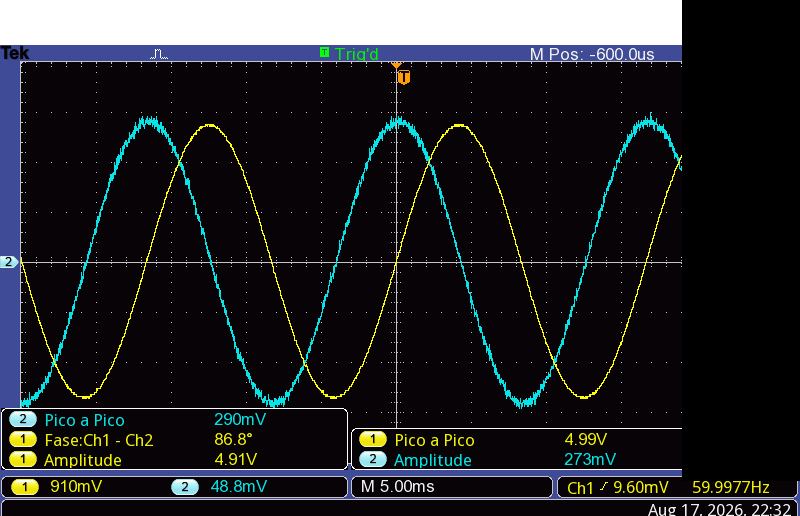
\includegraphics[width=0.31\linewidth]{figs/PA_60hz_cortada.png}}
	\subfigure[PA, $1000\,\text{Hz}$]{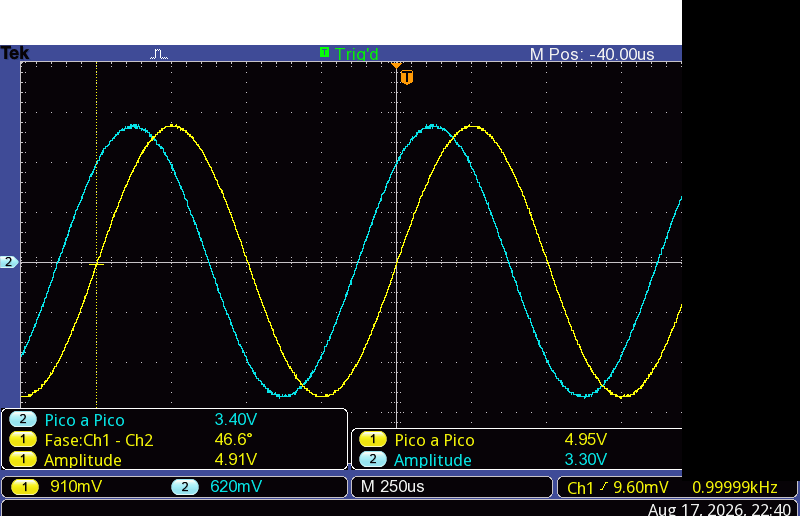
\includegraphics[width=0.31\linewidth]{figs/PA_1000hz_cortada.png}}
	\subfigure[PA, $20000\,\text{Hz}$]{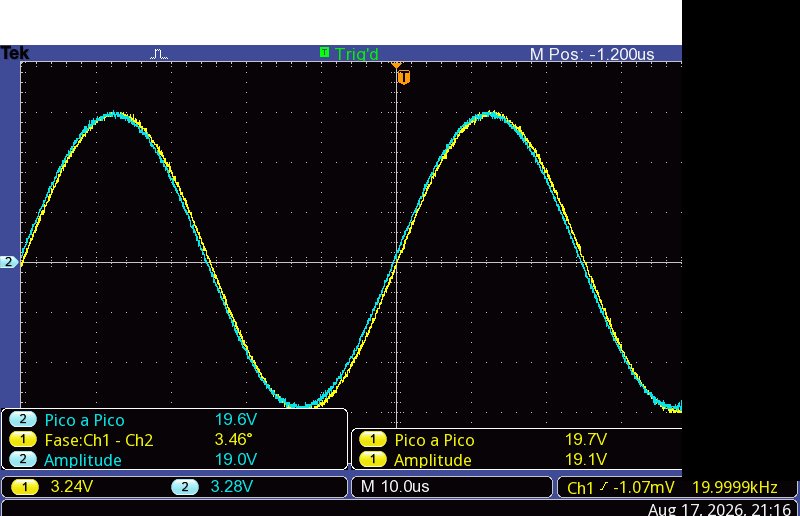
\includegraphics[width=0.31\linewidth]{figs/PA_20000hz_cortada.png}}
	\subfigure[PB, $60\,\text{Hz}$]{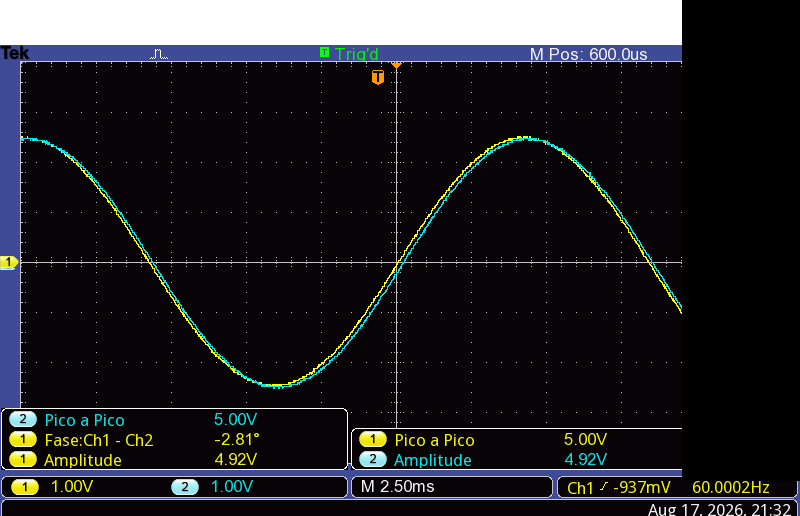
\includegraphics[width=0.31\linewidth]{figs/PB_60hz_cortada.png}}
	\subfigure[PB, $1000\,\text{Hz}$]{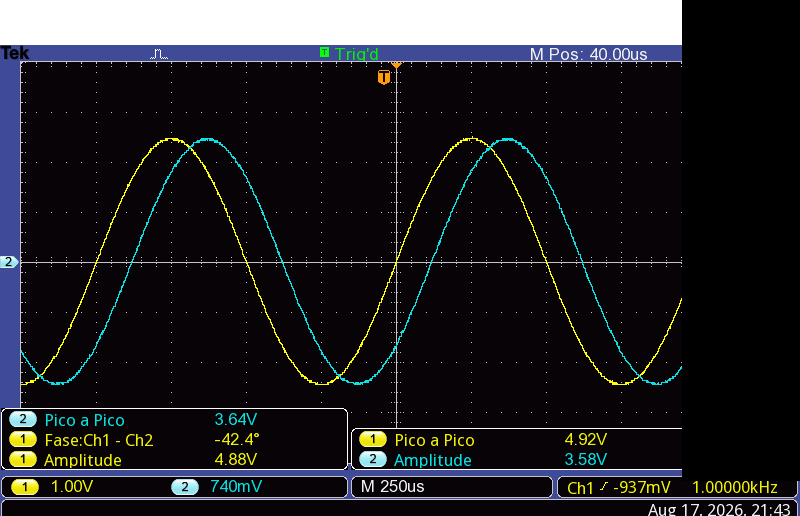
\includegraphics[width=0.31\linewidth]{figs/PB_1000hz_cortada.png}}
	\subfigure[PB, $20000\,\text{Hz}$]{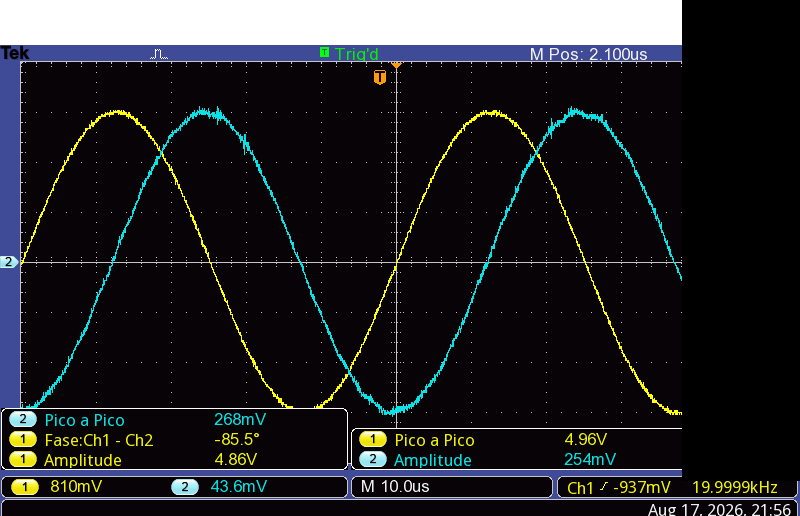
\includegraphics[width=0.31\linewidth]{figs/PB_20000hz_cortada.png}}
	\caption{\label{fig:telas} Telas do osciloscópio TBS 1052B-EDU (traço amarelo: $V_e$, Ch1; traço ciano: $V_s$, Ch2) para os filtros passa-altas (PA, a-c) e passa-baixas (PB, d-f) em três frequências representativas: bem abaixo, próximo e bem acima de $f_c\approx1061\,\text{Hz}$.}
\end{figure}

A Figura~\ref{fig:linear} apresenta as curvas de ganho e fase em escala linear (eixo de frequência logarítmico) e a Figura~\ref{fig:bode} apresenta o diagrama de Bode (ganho em dB), ambas com a curva teórica das Eqs.~\eqref{eq:ganho_pa}-\eqref{eq:ganho_pb} sobreposta aos pontos experimentais. Em ambos os filtros, os pontos medidos acompanham de perto a curva teórica em toda a década e meia de frequência estudada, confirmando o modelo de filtro RC de primeira ordem. A frequência de corte experimental, obtida por interpolação linear em $\log f$ do cruzamento com $-3\,\text{dB}$, foi de $1081\,\text{Hz}$ para o passa-altas e $1085\,\text{Hz}$ para o passa-baixas -- ambas dentro de $2\%$ do valor teórico $f_c=1061\pm119\,\text{Hz}$, portanto bem dentro da incerteza combinada.

\begin{figure}[htp]
	\centering
	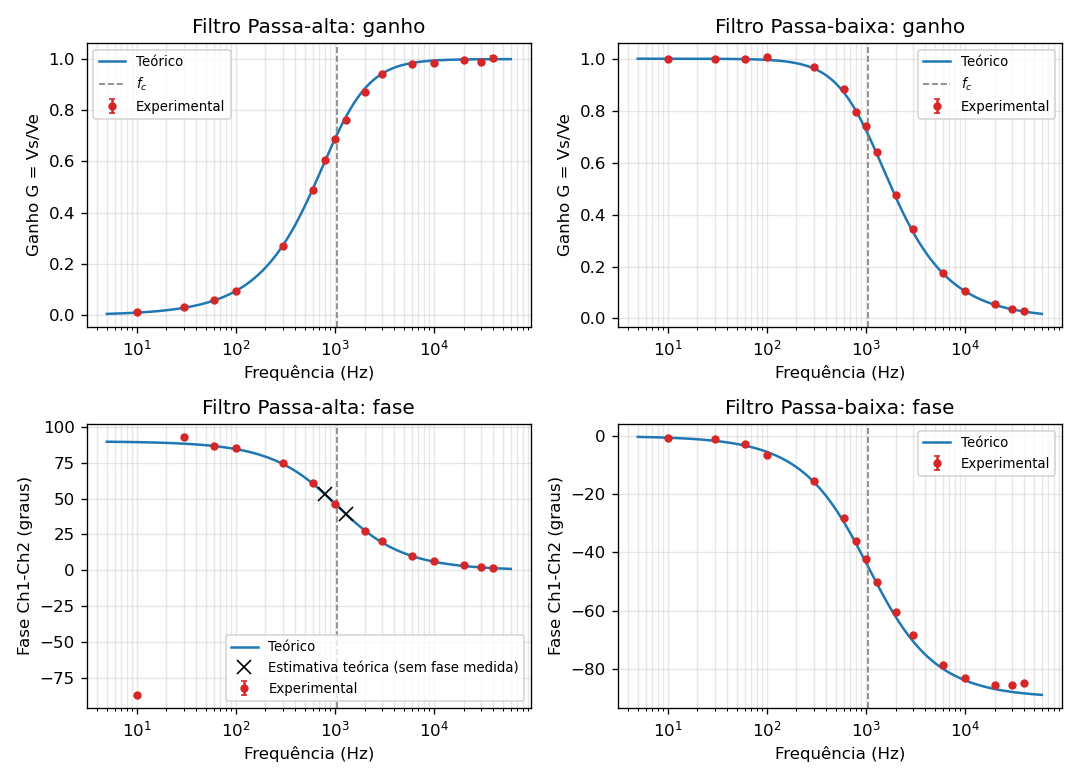
\includegraphics[width=\linewidth]{figs/resposta_linear.png}
	\caption{\label{fig:linear} Resposta em frequência em escala linear (eixo de frequência logarítmico) dos filtros passa-altas e passa-baixas: ganho $G=V_s/V_e$ (topo) e fase $\Phi$ (base). Os pontos marcados com $\times$ em $800$ e $1300\,\text{Hz}$ (PA) são a estimativa teórica de preenchimento, não uma medida.}
\end{figure}

\begin{figure}[htp]
	\centering
	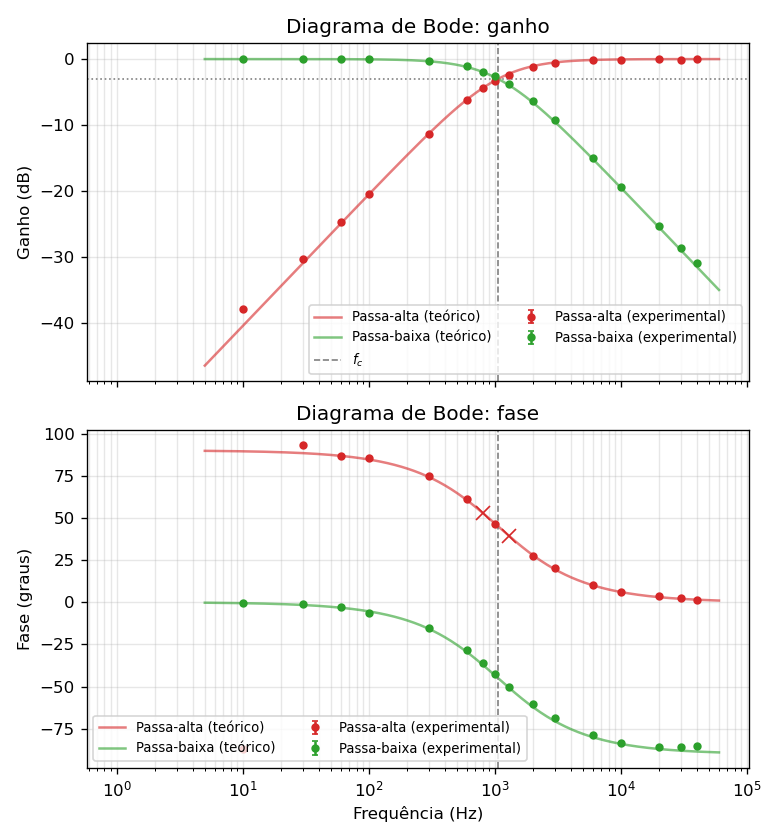
\includegraphics[width=\linewidth]{figs/bode.png}
	\caption{\label{fig:bode} Diagrama de Bode dos filtros passa-altas e passa-baixas: ganho em dB (topo, linha pontilhada em $-3\,\text{dB}$) e fase (base), com a frequência de corte teórica $f_c$ indicada pela linha vertical tracejada.}
\end{figure}

\begin{figure}[htp]
	\centering
	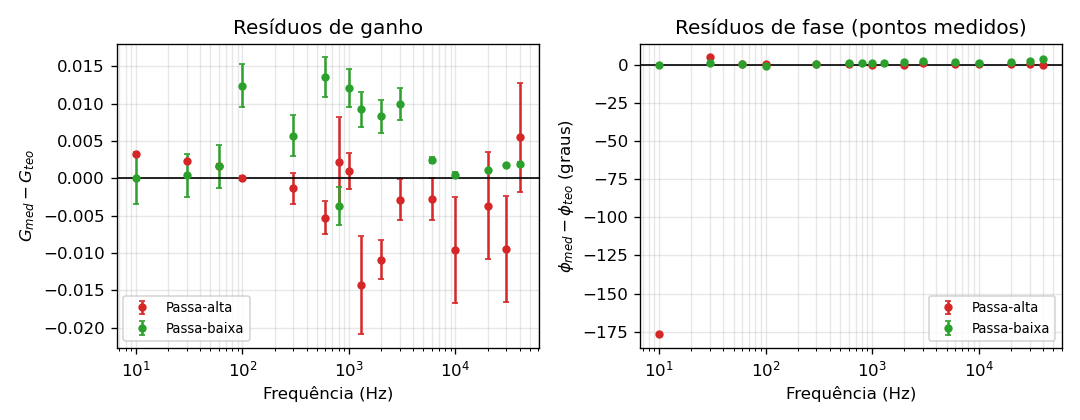
\includegraphics[width=\linewidth]{figs/residuos.png}
	\caption{\label{fig:residuos} Resíduos entre os valores medidos e o modelo teórico: ganho $G_{med}-G_{teo}$ (esquerda) e fase $\Phi_{med}-\Phi_{teo}$ nos pontos com defasagem medida (direita).}
\end{figure}

A Figura~\ref{fig:residuos} apresenta os resíduos entre os valores medidos e o modelo teórico. Os resíduos de ganho são pequenos e sem tendência sistemática clara em nenhum dos dois filtros (PA: média $-0{,}0028$, desvio padrão $0{,}0057$; PB: média $0{,}0048$, desvio padrão $0{,}0053$, ambos compatíveis com zero dentro de poucas vezes a incerteza de leitura). O maior resíduo de ganho individual ocorre exatamente nos dois pontos do PA sem defasagem medida ($800$ e $1300\,\text{Hz}$, resíduo até $0{,}014$), o que é consistente com esses dois pontos terem sido lidos do quadro "Amplitude" em vez de "Pico a Pico" nas capturas originais -- uma pequena diferença de algoritmo de medida do próprio instrumento, e não um efeito físico do circuito. Os resíduos de fase do PB são pequenos e crescem levemente com a frequência, de $-0{,}2^\circ$ em $10\,\text{Hz}$ até $+3{,}6^\circ$ em $40\,\text{kHz}$; essa tendência sistemática é compatível com uma pequena capacitância parasita do cabo/ponta de prova não incluída no modelo ideal, que se torna relativamente mais importante em alta frequência.

O ponto de $10\,\text{Hz}$ do filtro passa-altas apresenta um resíduo de fase anômalo e grande em módulo ($\approx-176^\circ$): a fase medida tem sinal negativo ($-86{,}8^\circ$), destoando da tendência positiva decrescente dos demais dez pontos do PA ($93^\circ$ a $1{,}4^\circ$) e do valor teórico ($+89{,}5^\circ$ nessa frequência). Em módulo, a concordância é boa ($|{-86{,}8}|-89{,}5=-2{,}7^\circ$), da mesma ordem dos demais resíduos. A imagem de origem mostra o traço de $V_s$ visivelmente ruidoso, compatível com uma tensão de saída muito pequena ($52\,\text{mV}$, próxima do piso de ruído do osciloscópio na escala usada); nessas condições, o algoritmo de medida automática de fase do instrumento é suscetível a ambiguidade de sinal, o que é a explicação mais provável para essa inversão isolada -- não um erro sistemático de conexão dos canais, já que os demais nove pontos do PA (incluindo $30\,\text{Hz}$, também com defasagem próxima de $90^\circ$) mantêm o sinal positivo esperado. Optou-se por manter o valor medido na Tabela~\ref{tab:pa} e discutir a discrepância abertamente, em vez de descartá-la.

Por fim, dois pontos do filtro passa-altas ($800$ e $1300\,\text{Hz}$) não têm defasagem medida: as capturas de tela correspondentes foram salvas com o quadro "Amplitude" aberto em vez do quadro "Fase:Ch1-Ch2", e nenhuma captura alternativa com a defasagem foi encontrada para essas duas frequências (inclusive um segundo conjunto de imagens fornecido posteriormente foi conferido por soma de verificação e mostrou ser cópia idêntica do primeiro). Os valores de fase mostrados nas Tabelas~\ref{tab:pa} e na Figura~\ref{fig:linear} para esses dois pontos são, portanto, a estimativa teórica da Eq.~\eqref{eq:ganho_pa}, e não uma medida -- indicados explicitamente com $^\dagger$ na tabela e com $\times$ no gráfico.

\section{Conclusão}

As curvas de resposta em frequência de ganho e fase de filtros RC passa-altas e passa-baixas ($R=1{,}5\,\text{k}\Omega$, $C=0{,}1\,\mu\text{F}$ nominais) foram determinadas experimentalmente para 16 frequências entre $10\,\text{Hz}$ e $40\,\text{kHz}$ e mostraram excelente concordância com o modelo de impedância complexa em toda a faixa estudada, com resíduos de ganho tipicamente abaixo de $1\%$ e de fase abaixo de $1^\circ$ na maioria dos pontos. A frequência de corte experimental, $1081\,\text{Hz}$ (PA) e $1085\,\text{Hz}$ (PB), concorda com o valor teórico $f_c=1061\pm119\,\text{Hz}$ dentro de $2\%$, bem dentro da incerteza combinada, validando o modelo $f_c=1/(2\pi RC)$. Duas limitações de coleta foram identificadas e discutidas: os pontos de $800$ e $1300\,\text{Hz}$ do PA não tiveram a defasagem capturada e foram preenchidos com a estimativa teórica, marcada explicitamente como tal; e o ponto de $10\,\text{Hz}$ do PA apresentou uma provável inversão de sinal na medida automática de fase, atribuída ao baixo nível de sinal e alto ruído nessa condição, mas com boa concordância em módulo. Um leve resíduo sistemático crescente com a frequência foi observado na fase do PB, possivelmente associado a capacitância parasita não modelada. Em conjunto, os resultados confirmam o comportamento esperado de filtro passa-altas e passa-baixas de primeira ordem previsto pelas Eqs.~\eqref{eq:ganho_pa}-\eqref{eq:ganho_pb}.

\section*{Referências}
\bibliographystyle{apsrev4-2}

\bibliography{library}

\end{document}
